\documentclass[10pt,a4paper]{article}
\usepackage[english]{babel}
\usepackage[utf8]{inputenc}
\usepackage{amsmath}
\usepackage{amsfonts}
\usepackage{amssymb}
\usepackage{graphicx}
\usepackage{float}

%link to documentation: 
%https://ackrep-doc.readthedocs.io/en/latest/devdoc/contributing_data.html

\begin{document}
	\part*{Model Documentation of the \\ Winkler System} % MUST - Add Model Name 
	
	%%%%%%%%%%%%%%%%%%%%%% NOMENCLATURE %%%%%%%%%%%%%%%%%%%%%%%%%%%
	
	\section{Nomenclature} % MUST
	\subsection{Nomenclature for Model Equations} % MUST
	
	%variables for model equations
	\begin{tabular}{ll}
		$x$ & x-coordinate \\
		$y$ & y-coordinate \\
		
				
	\end{tabular}
	 
	
	%variables which are used additional to those in the model equations
	\begin{tabular}{ll}

	\end{tabular}
	
	%%%%%%%%%%%%%%%%%%%%%% MDOEL EQUATIONS %%%%%%%%%%%%%%%%%%%%%%%%%%%
	
	\section{Model Equations} % MUST
	
	State Vector:
	\begin{align*}
		\underline{x} &= (x \ y)^T &= (x_1 \ x_2)^T 
	\end{align*}
	
	\noindent System Equations:			
	\begin{subequations}
	\begin{align}
		\dot{x}_1 &= 2x_2 \\
		\dot{x}_2 &= (x_1 + x_2)(-(x_1 - x_2)^2 + 1)
	\end{align}
	\end{subequations}

	
	%%%%%%%%%%%%%%%%%%%%%% ASSUMPTIONS %%%%%%%%%%%%%%%%%%%%%%%%%%%
	

	%%%%%%%%%%%%%%%%%%%%%% DERIVATION & EXPLANATION %%%%%%%%%%%%%%%%%%%%%%%%%%%	
	
	\section{Derivation and Explanation} % SHOULD
	The Winkler System is nonlinear and unstable. It has three rest positions, one spiral source in (-1, 0), one spiral source in (1, 0) and one saddle point in (0, 0). You can recognize the symmetry to the point of origin. 
	\begin{figure}[H]
		\centering
		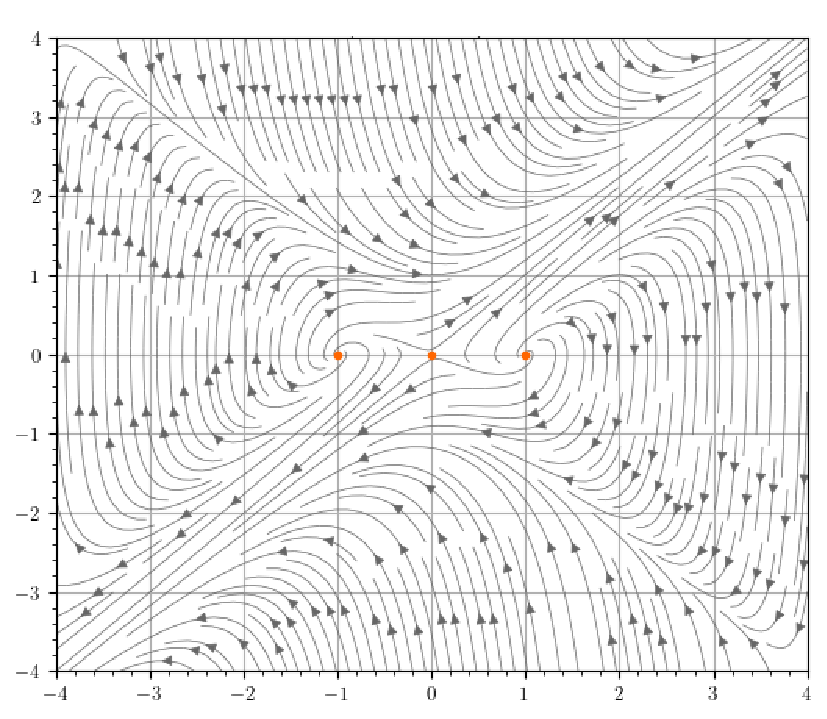
\includegraphics[width=70mm]{winkler_pp.pdf}
		\caption{Phaseplane}
	\end{figure}
	
	%%%%%%%%%%%%%%%%%%%%%% REFERENCES %%%%%%%%%%%%%%%%%%%%%%%%%%%
	
	\begin{thebibliography}{10}		
		\bibitem{But21}Winkler, Jan:
		\textit{Lecture Notes "Nonlinear Control Systems 1"}, Institut of Control Theory TU Dresden, published 2022.
	\end{thebibliography}

\end{document}

